\section{Automated evaluation}
In \Cref{alg:converse_algo}, we show the user-agent self-play procedures that we used to perform all automated evaluation.

\begin{figure}[h]
  \centering
  \begin{minipage}{0.49\textwidth}
    \centering
    \textbf{ImageInWords T2T DSG} 
    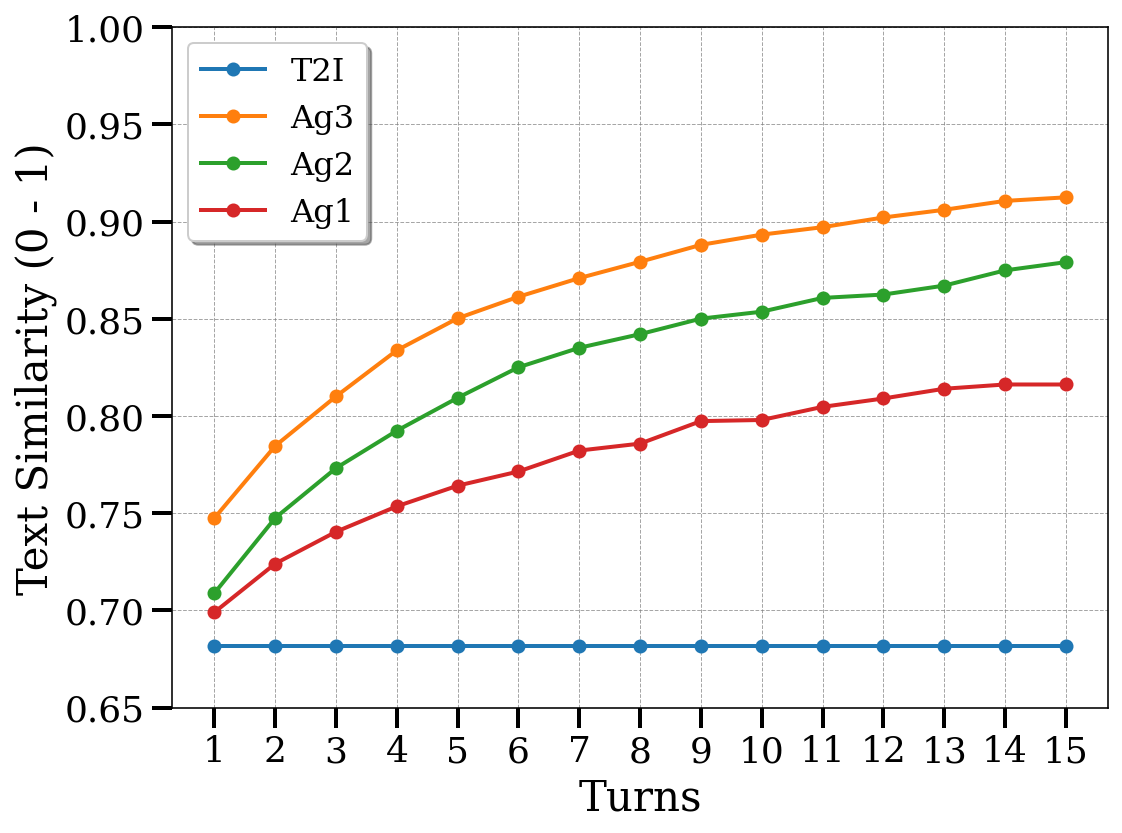
\includegraphics[width=\linewidth]{figures/imageinwords_dsgt2t.png}
  \end{minipage}
  \hfill
  \begin{minipage}{0.49\textwidth}
    \centering
    \textbf{Coco Captions T2T DSG} 
    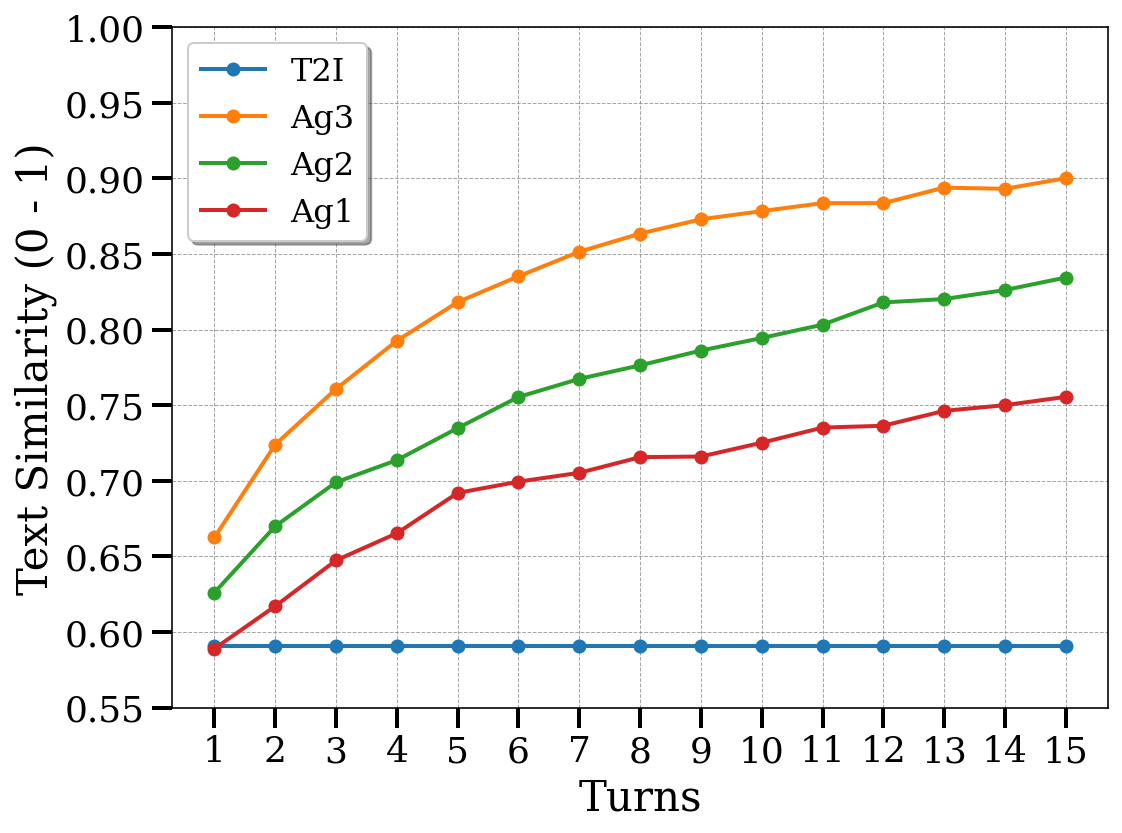
\includegraphics[width=\linewidth]{figures/coco_captions_dsgt2t.png}
  \end{minipage}
  \begin{minipage}{0.49\textwidth}
    \centering
    \textbf{DesignBench T2T DSG} 
    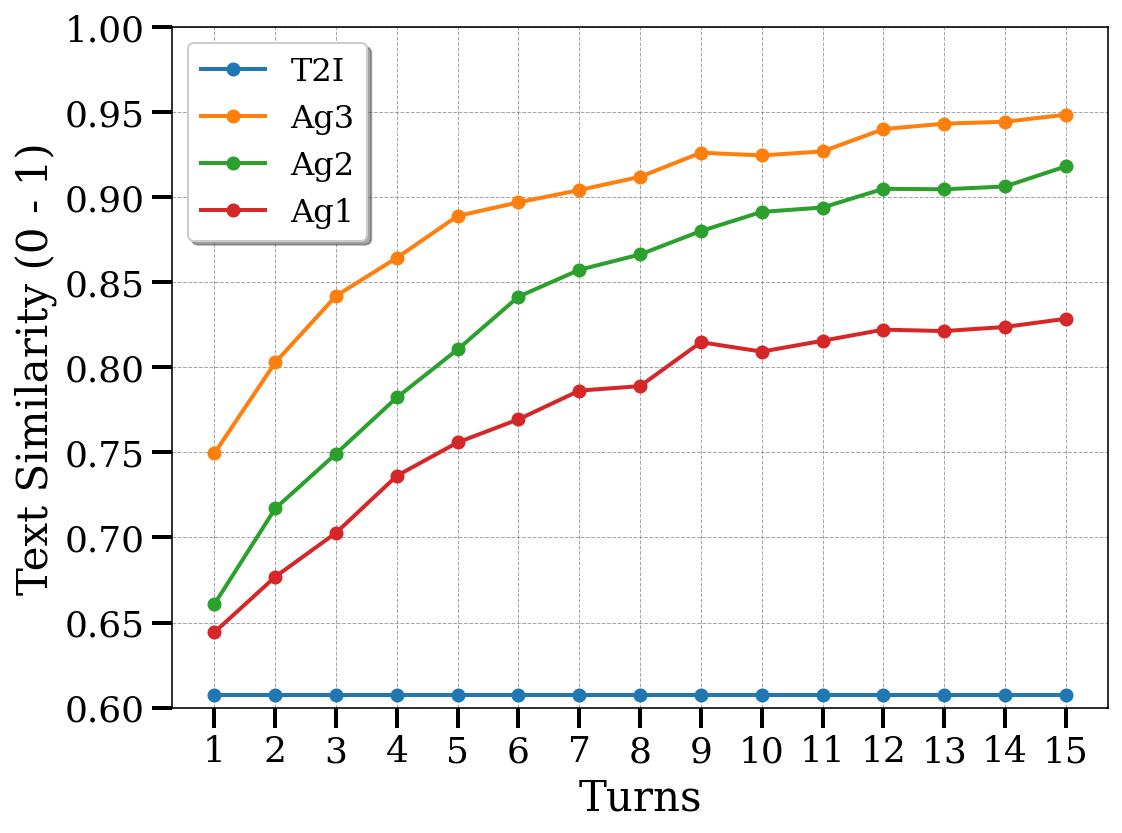
\includegraphics[width=\linewidth]{figures/toy_dataset_dsgt2t.png}
  \end{minipage}
  \caption{DSG score comparison between ground truth prompt and agent generated prompt reported at each turn. The performance of all agents increase with increase in number of turns.}
  \label{fig:dsg_figures}
\end{figure}


\begin{algorithm}[t]
\caption{User-Agent Self-Play Algorithm \nitkan{we can make this half page and wrap text around this. Not sure how, can someone try this?}}
\label{alg:converse_algo}
\begin{algorithmic}[1] 
\STATE \textbf{Input:} Initial prompt $p_0$, User $u$, Agent $a$ (with $p_0$), $max\_turns$
\STATE \textbf{Output:} Refined prompt $p_f$ 
\STATE $p_f \gets p_0$ 
\FOR{$turn\_id = 0$ \TO $max\_turns - 1$}
    \STATE $action \gets a.\text{SelectAction}()$
    \STATE $question \gets a.\text{VerbalizeAction}(action)$
    \STATE $answer \gets u.\text{AnswerQuestion}(question)$
    \STATE $a.\text{Transition}(action, answer)$
    \STATE $p_f \gets a.prompt$
\ENDFOR
\RETURN $p_f$
\end{algorithmic}
\end{algorithm}
